
\section{Motivation}
% --- Section 0: Introduction ---
\begin{frame}{Why Learn This?}
    \pause
    \begin{minipage}{0.45\textwidth}
        \centering
        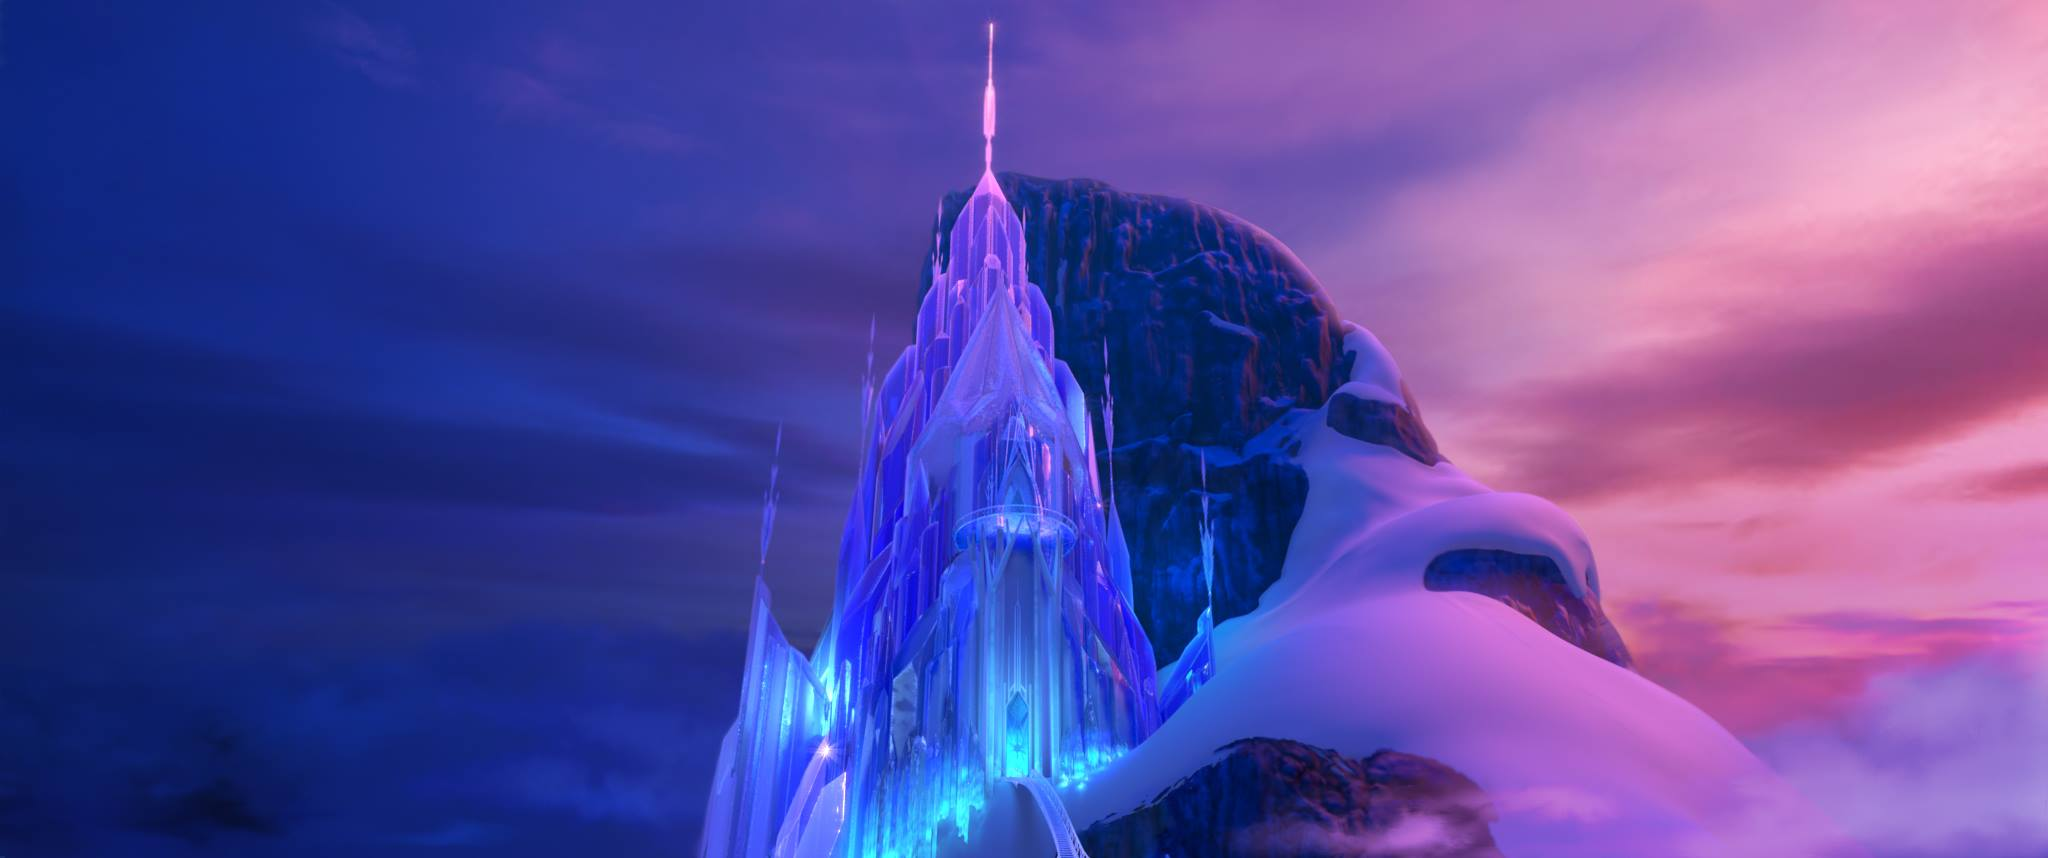
\includegraphics[width=\linewidth]{images/frozen_castle.jpg}
        \captionof*{figure}{Elsa's Castle in Frozen}
    \end{minipage}%
    \hfill
    \pause
    \begin{minipage}{0.45\textwidth}
        \centering
        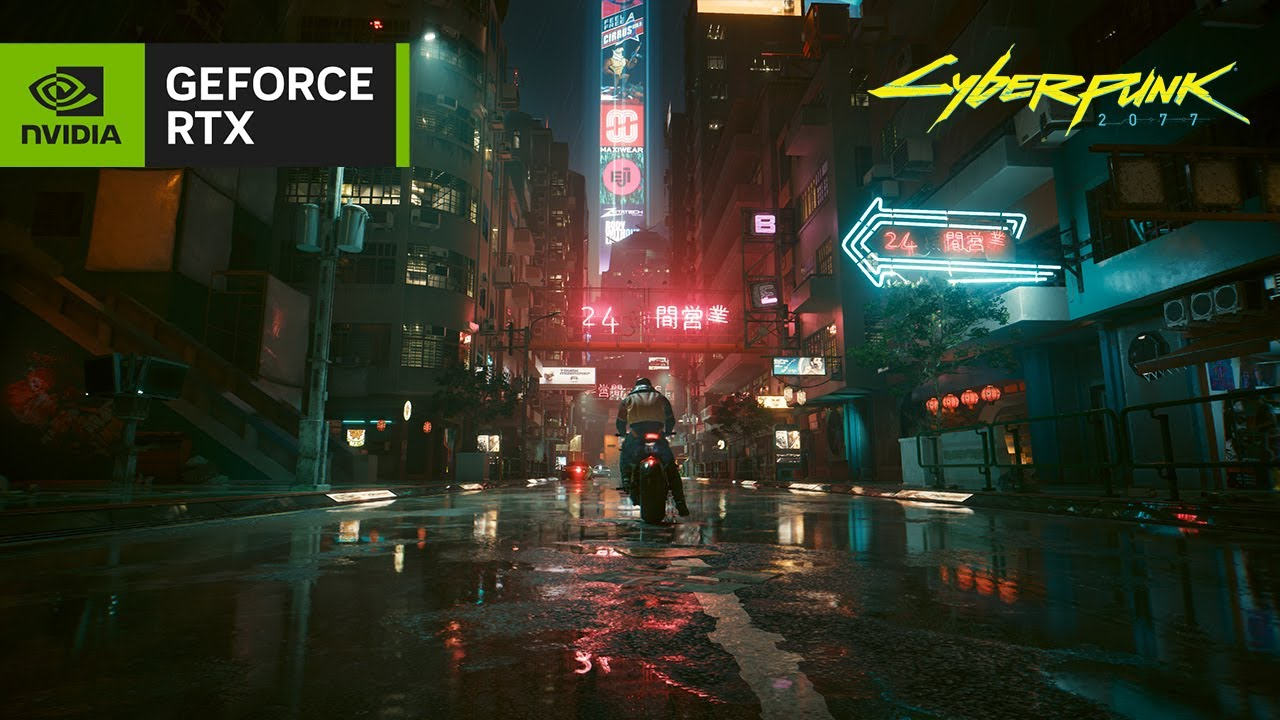
\includegraphics[width=\linewidth]{images/cyberpunk_rtx.jpg}
        \captionof*{figure}{ Cyberpunk 2077 with RTX}
    \end{minipage}

    \begin{itemize}
        \item<3-> \textbf{Realistic graphics} of your favourite animated movies are the result of ground-breaking work in Ray Tracing by
              studios like Disney, Pixar, and DreamWorks. Do you know these films take years to render? 30 hours per frame!
        \item<4-> Lately, \textbf{RTX} is all the rage in gaming. New titles boast ray-tracing effects in real-time, not 30 hours per frame!
        \item<5-> It's fun! You will know when you create your first ray-traced image!
    \end{itemize}
\end{frame}

% --- Section 1: The Story Begins ---
\section{The Story of Light}

\begin{frame}{How Do We See?}
    \begin{columns}
        \begin{column}{0.5\textwidth}
            \begin{tikzpicture}[scale=0.8]
                % Sun
                \node[circle, fill=LightColor, minimum size=1cm] (sun) at (0,3) {\faIcon{sun}};
                \node[below] at (0,4.25) {\small \textcolor{LightColor}{Light Source}};
                \draw[lightray] (sun) -- (2,1);
                \draw[lightray] (sun) -- (3,2);
                \draw[lightray] (sun) -- (4,1);

                % Object
                \node[sphere] (obj) at (3,1) {};

                % Eye
                \node[eye] (eye) at (5,3) {\faIcon{eye}};
                \draw[reflectray] (3.1,2) -- (eye);

                \node[below] at (3,0) {\small \objectcolor{Object}};
                \node[below] at (5,4.1) {\small \textcolor{PrimaryColor}{Observer}};
            \end{tikzpicture}
        \end{column}
        \pause
        \begin{column}{0.5\textwidth}

            \only<2>{
                \begin{conceptbox}{Natural Process}
                    \begin{enumerate}
                        \item Light travels from source
                        \item Light hits objects
                        \item Light bounces to our eyes
                        \item Our brain interprets the signal
                    \end{enumerate}
                \end{conceptbox}
            }

            \only<3>{
                \begin{conceptbox}{Physical Process}
                    \begin{enumerate}
                        \footnotesize
                        \item Photon is emitted from source
                        \item Photon hits objects
                        \item Part of the photon is reflected or absorbed
                        \item The reflected photons reach our eyes
                        \item The rods and cones in our retina detect the photons
                        \item Our brain interprets the signal
                        \item \textbf{Colour}: The wavelength of the photons
                        \item \textbf{Brightness}: The number of photons
                    \end{enumerate}
                \end{conceptbox}
            }

            \only<4>{
                \vspace{0.5cm}
                \alert{Question:} How do we simulate this?
            }

        \end{column}
    \end{columns}
\end{frame}

\begin{frame}{The Computer Graphics Challenge}
    \begin{center}
        \begin{tikzpicture}[scale=0.9]
            % Real world
            \node[rectangle, draw, minimum width=3cm, minimum height=2cm, fill=LightGray] (real) at (0,0) {\faIcon{globe} Real World};
            \node[above] at (0,1.5) {\textbf{Infinite Complexity}};

            % Computer
            \node[rectangle, draw, minimum width=3cm, minimum height=2cm, fill=PrimaryColor!20] (comp) at (5,0) {\faIcon{laptop} Computer};
            \node[above] at (5,1.5) {\textbf{Finite Pixels}};

            % Arrow
            \draw[->, very thick, AccentColor]
            (real.east) -- (comp.west)
            node[midway, above, text=AccentColor, font=\footnotesize]{Simulate};


            % Challenges
            \node[below] at (2.5,-2  ) {
                \begin{minipage}{6cm}
                    \textcolor{AccentColor}{\textbf{Challenges:}}
                    \begin{itemize}
                        \item Infinite light rays/photons
                        \item Complex physics
                        \item High computational cost
                    \end{itemize}
                \end{minipage}
            };
        \end{tikzpicture}
    \end{center}
\end{frame}

% --- Section 2: Ray Casting ---
\section{Ray Casting: Foundation}

\begin{frame}{The Key Insight}
    \begin{columns}
        \begin{column}{0.5\textwidth}
            \begin{raybox}{1. Reverse Engineering}
                Instead of following light rays from light sources |

                \vspace{0.1cm}
                \textbf{Let's trace backwards!}

                \textbf{Shoot rays from the eye}, find where it hits and find out how much light reaches there.
            \end{raybox}

            \vspace{0.3cm}
            This is the opposite of what happens in reality.
            \textbf{Why does this work?}
            \begin{itemize}
                \small
                \item<2-> Most light never reaches our eyes
                \item<3-> Only trace rays that matter
                \item<3-> Much more efficient!
            \end{itemize}
        \end{column}
        \begin{column}{0.5\textwidth}
            \begin{tikzpicture}[scale=0.6]
                % Define 3D styles
                \tikzset{
                    screen/.style={fill=blue!10, draw=blue!50, opacity=0.8},
                    pixel/.style={fill=AccentColor!60, thick},
                    primary ray/.style={->, very thick, red!90},
                    object/.style={fill=orange!60, draw=orange!80, circle, minimum size=12pt}
                }

                % Eye position in 3D space

                \node[eye] (eye) at (0,0,0) {\faIcon{eye}};
                % Object in 3D space
                \node[sphere, minimum size=1cm] (obj) at (8,0,3.8) {};

                % Labels
                \node[below] at (0,-0.6,0) {\small Eye};
                \node[below] at (8,-1,3.8) {\small \objectcolor{Object}};

                \node[circle, fill=LightColor, minimum size=1cm] (sun) at (5,3.5) {\faIcon{sun}};
                \node[below] at (5,5) {\small \textcolor{LightColor}{Light Source}};

                \draw[ray, very thick] (eye.center) -- (obj.west);
                \draw[ray, thick, opacity=0.5] (obj.west) -- ($(sun.south) + (0,0,0)$);
                \draw[ray, thick, opacity=0.5] (obj.west) -- ($(sun.south) + (0,-0.2,-1)$);
                \draw[ray, thick, opacity=0.5] (obj.west) -- ($(sun.south) + (0,-0.3,-2)$);
                \draw[ray, thick, opacity=0.5] (obj.west) -- ($(sun.south) + (0,0.5,1)$);
                \draw[ray, thick, opacity=0.5] (obj.west) -- ($(sun.south) + (0,1.2,2)$);


                \pause

                \only<2> {
                    \draw[ray, black!50, thick, opacity=0.8, dashed] (sun) -- (obj.north);
                    \draw[ray, black!50, thick, opacity=0.8, dashed] (obj.north) -- (8,2)
                    node[above] {\small \textcolor{black!50}{Useless ray}};
                }

                \pause

            \end{tikzpicture}
        \end{column}
    \end{columns}
\end{frame}


\begin{frame}{From Infinite Rays to Finite Pixels}
    \begin{columns}
        \begin{column}{0.6\textwidth}
            \begin{raybox}{2. Cutting Costs}
                Instead of tracing infinite rays |

                \vspace{0.1cm}
                \textbf{Trace one ray per pixel.}
            \end{raybox}
            \vspace{0.3cm}
            This comes with little tradeoff, because:
            \begin{itemize}
                \small
                \item<2-> An image is just a grid of pixels
                \item<3-> Each pixel can only be of one color
                \item<4-> In the end, we just need to know the \emph{color of each pixel}
                \item<5-> Hence, one ray from the mid-point of each pixel should be a good approximation$^*$ \\
            \end{itemize}
            \vspace{0.3cm}
            \begin{itemize}
                \footnotesize
                \item<5->[$^*$] We will discuss more advanced techniques later that improve quality
            \end{itemize}
        \end{column}
        \begin{column}{0.4\textwidth}
            \centering
            \pause
            \begin{tikzpicture}[scale=0.6]
                % Define 3D styles
                \tikzset{
                    screen/.style={fill=blue!10, draw=blue!50, opacity=0.8},
                    pixel/.style={fill=AccentColor!60, thick},
                    primary ray/.style={->, very thick, red!90},
                    object/.style={fill=orange!60, draw=orange!80, circle, minimum size=12pt}
                }

                \fill[screen] (-3,-3) rectangle (3,3);


                \foreach \x in {-3,-2,...,3} {
                        \draw[gray!60, thin] (\x,-3) -- (\x,3);
                    }
                \foreach \z in {-3,-2,...,3} {
                        \draw[gray!60, thin] (-3,\z) -- (3,\z);
                    }


                \pause
                \fill[pixel] (-2,-2) rectangle (-1,-1);

                \pause
                \pause

                \foreach \x in {-2.5,-1.5,...,2.5} {
                        \foreach \z in {-2.5,-1.5,...,2.5} {
                                \fill[red!70] (\x, \z) circle (0.1);
                            }
                    }


            \end{tikzpicture}
        \end{column}
    \end{columns}
\end{frame}


\begin{frame}{The Full Picture}
    \begin{columns}
        \begin{column}{0.5\textwidth}
            \begin{tikzpicture}[node distance=1.2cm]
                \node<2->[process] (screen) {Place screen in front of eye};
                \node<3->[process, below of=screen] (start) {For each pixel};
                \draw<3->[arrow] (screen) -- (start);

                \node<4->[process, below of=start] (ray) {Shoot ray from eye};
                \draw<4->[arrow] (start) -- (ray);

                \node<5->[process, below of=ray] (intersect) {Find closest intersection};
                \draw<5->[arrow] (ray) -- (intersect);

                \node<6->[process, fill=AccentColor!50, below of=intersect] (shade) {Calculate color$^*$};
                \draw<6->[arrow] (intersect) -- (shade);

                \node<7->[process, below of=shade] (end) {Set pixel color};
                \draw<7->[arrow] (shade) -- (end);

                \draw<8->[arrow] (end) -- ($(end)+(-2.25,0)$) |- (start);
            \end{tikzpicture}
        \end{column}
        \begin{column}{0.5\textwidth}
            \begin{tikzpicture}[scale=0.6]
                % Define 3D styles
                \tikzset{
                    screen/.style={fill=blue!10, draw=blue!50, opacity=0.8},
                    pixel/.style={fill=AccentColor!60, thick},
                    primary ray/.style={->, very thick, red!90},
                    object/.style={fill=orange!60, draw=orange!80, circle, minimum size=12pt}
                }
                % Eye position in 3D space
                \node[eye] (eye) at (0,0,0) {\faIcon{eye}};
                % Object in 3D space
                \node[sphere, minimum size=1cm] (obj) at (8,0,3.8) {};
                % Labels
                \node[below] at (0,-0.6,0) {\small Eye};
                \node[below] at (8,-1,3.8) {\small \objectcolor{Object}};
                \node[circle, fill=LightColor, minimum size=1cm] (sun) at (5,3.5) {\faIcon{sun}};
                \node[below] at (5,5) {\small \textcolor{LightColor}{Light Source}};
                \pause
                \node[below] at (3.5,-4,0) {\small Screen};
                \only<6->{
                    \draw[ray, thick, opacity=0.3] (obj.west) -- ($(sun.south) + (0,0,0)$);
                    \draw[ray, thick, opacity=0.3] (obj.west) -- ($(sun.south) + (0,-0.2,-1)$);
                    \draw[ray, thick, opacity=0.3] (obj.west) -- ($(sun.south) + (0,-0.3,-2)$);
                    \draw[ray, thick, opacity=0.3] (obj.west) -- ($(sun.south) + (0,0.5,1)$);
                    \draw[ray, thick, opacity=0.3] (obj.west) -- ($(sun.south) + (0,1.2,2)$);
                }
                % Screen plane in 3D (using canvas is plane)
                \begin{scope}[canvas is zy plane at x=3.5]
                    % Background screen
                    \fill[screen] (-3,-3) rectangle (3,3);
                    \foreach \x in {-3,-2,...,3} {
                            \draw[gray!60, thin] (\x,-3) -- (\x,3);
                        }
                    \foreach \z in {-3,-2,...,3} {
                            \draw[gray!60, thin] (-3,\z) -- (3,\z);
                        }
                    \pause
                    \fill[pixel] (-2,-2) rectangle (-1,-1);
                    \pause
                    \fill[red!70] (-1.5, -1.5) circle (0.1);
                    \draw<5->[ray, very thick] (eye.center) -- (-1.5, -1.5);
                    \draw<5->[->, ray, very thick] (-1.5, -1.5) -- (obj);
                    \pause
                    \pause
                    \pause
                    \fill[RayColor!60] (-2,-2) rectangle (-1,-1);
                    \fill[red!70] (-1.5, -1.5) circle (0.1);
                    \pause
                    \foreach \x in {-2.5,-1.5,...,2.5} {
                            \foreach \z in {-2.5,-1.5,...,2.5} {
                                    \fill[red!70] (\x, \z) circle (0.1);
                                    \draw[ray, thick, opacity=0.3] (eye.center) -- (\x,\z);
                                }
                        }
                \end{scope}
                \draw<4>[->, ray, very thick] (eye) -- ($(obj) + (3.5, 0, 1.5)$);
            \end{tikzpicture}
        \end{column}
    \end{columns}
\end{frame}
